\chapter{Classification: Alternative Techniques}
	
	A {\bf Instance based} classifiers is based on the concept of "instance" and store
	the training records. It uses the training records to predict the plass label
	of unseen cases. It does not build a model in the strict sence as a decision tree. 

	{\bf Rote-learner:}
	\begin{itemize}
		\item Memorizes entire training data
		\item Performs classification only if attributes of record match
		one of the training exactly
	\end{itemize}

	In this section we will capture these algorithms: 
	\begin{itemize}
		\item Instance-based learning: k-NN
		\item Probabilistic learning: Naive Bayes
		\item Statistical learning: Support Vector Machines (SVM)
	\end{itemize}


	
	\clearpage
	\section{Nearest-Neighbor Classifiers}

		Decision tree classifier are an example of {\bf eager learner} because
		they are designed to learn a model that maps the input attributes to 
		the class label as soon as the training data becomes available. 
		An opposite strategy would be to delay the process of modeling the 
		training data until it is needed to classify the test examples.
		Techniques that employ this strategy are known as {\bf lazy learners}.

		An obvious drawback of this approach is that some test records may not
		be classified because they do not match any training example. 
		One way to make this approach more flexible is to find all the
		training examples that are relatively similar to the attribues of the
		test example. These examples are known as {\bf nearest neighbors}.

		\vspace{0.3cm}
		{\it \Large "If it walks like a duck , quacks like a duck, and looks like a duck,
		then it's probably a duck."}

		\vspace{0.3cm}

		A nearest-neighbor classifier represents each example as a data point
		in a d-dimensional space, where d is the number of attributes. 
		The k-nearest neighbors of a given example {\it z} refer to the
		{\it k} points that are close to {\it z}.
		To classify an example it uses the {\bf majority} of classes closest to the point.

		In the picture below you can see K-nearest neighbors of a record x are data 
		points that have the k smallest distance to x. In the first picture, x will
		be classified as "negative" because the majority is "negative".
		In the second picture will be classified as "positve".
		In this situation when it is a {\bf tie}, we choose randomly. 
		In the last picture	we classify x as "positive" because the majoiry is "positive"
		
		\begin{figure}[H]
			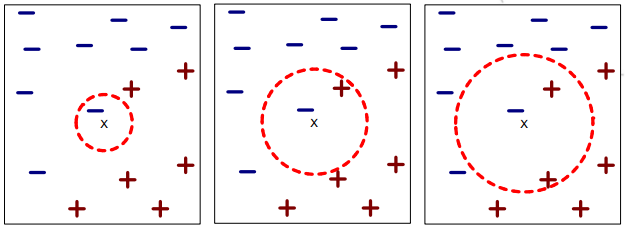
\includegraphics[width=\textwidth]{pics/knearest.png}
			\caption{1-nearest neighbor, 2-nearest neighbor and 3-nearest neighbor}
		\end{figure}

		You need to carefully pick the k because if its too small it can be close to noise
		so the classification is wrong. If the k is too big, it might happend that it
		will misclassify the test instance becuase its list of nearest neighbors may include
		data points that are located far away from its neighborhood.

		\clearpage
		\section{How to do the nearest-neighbor classifier}
		{\bf The nearest-Neighbor Classifier algorithm needs:}
			\begin{itemize}
				\item The set of stored records 
				\item Distance Metric to compute 
				\item distance between records
				\item The value of k, the number of nearest neighbors to retrieve 
			\end{itemize}
		{\bf To classify an unknown record you need to:}
			\begin{itemize}
				\item Compute distance to other training records
				\item Identify k nearest neighbors 
				\item Use class labels of nearest neighbors to determine the class 
				label of unknown record (e.g., by taking majority vote)
			\end{itemize}

		{\bf Calculate the distance between two points usin the Euclidean distance:}
		\begin{equation}
			Euclidean distance = d(p,q) = \sum_{i}^{} \sqrt{(p_{i} - q_{i})^{2}}
		\end{equation}

		\clearpage
	\section{Naive Bayes Classifier}

		In many applications the relationship between the attribute set and the class
		variable is {\bf non-deterministic}. In other words, the class label of a test
		record cannot be predicted with certainty even though its attribute set is 
		identical to some of the training examples. 

		This section presents an approach for modeling probilistic relationships
		between the attribute set and the class label. 

		Equations from probability theroy:
		\begin{equation}
			P(X,Y) = P(Y|X) \times P(X) = P(X|Y) \times P(Y)
		\end{equation}

		\begin{equation}
			P(Y|X) = \frac{P(X|Y)P(Y))}{P(X)}
		\end{equation}

		Let X denote the attribute set and Y denote the class variable. If the class variable
		has a non-deterministic relationship with the attributes, then we can treat X and Y
		as random variables and capture their relationships probabilistically using $P(Y|X)$.
		This conditional probability is also known as the {\bf posterior probability} for Y. 
		({\bf Prior probability} for Y is P(Y)).

		During the training phase, we need to learn the posterior probablities P(Y|X) for every
		combination of X an Y based on information gathered from the training data. 

		\begin{figure}[H]
			\centering
			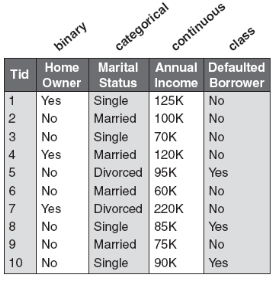
\includegraphics[scale=0.55]{pics/bayesian.png}
			\caption{Training set for predicting the loan default problem}
		\end{figure}

		Suppose we are given a test record with the following attribute set:

		X=(Home Owner = no, Marital Status = Married, Annual Income = 120K).

		To classify the record, we need to compute the posterior probabilities
		$P(Yes|X)$ and $P(No|X)$ based on the information available in the training data.
		If $P(Yes|X) > P(No|X)$, then the record is classified as Yes, otherwise it is classified
		as No. 

		When comparing the posterior probabilities for different values of Y, the denominator term
		{\bf P(X)}, is always {\bf constant}, and thus, can be ignored. 
		The prior probability {\bf P(Y)} can be easily estimated from the training set by computing
		the fraction of training records that belong to each class.	

		A naive Bayes classifier estimates the class-conditional probability by assuming 
		that the attributes are {\bf conditionally independent}, given the class variable y. 
		The assumption of conditionally independence of the attributes is the reason why P(X)
		can be ignored!

		\subsection*{Example: Play Tennis data}

		\begin{figure}[H]
			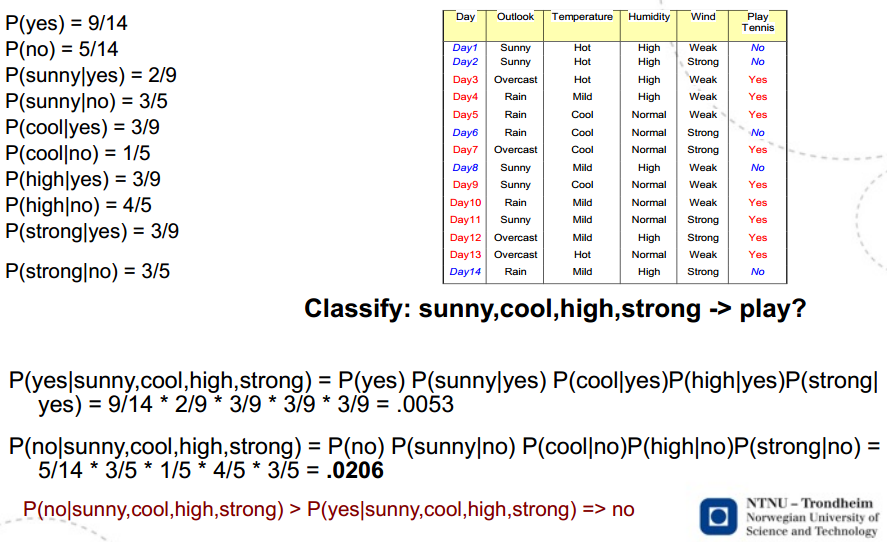
\includegraphics[width=\textwidth]{pics/examplenaive.png}
		\end{figure}

		\subsection{Estimating Conditional Probabilities for Continuous Attributes}

			There are two ways to estimate the class-conditional probabilities for 
			continuous attributes:

			\subsection*{1) Discretization}

				We can discretize each continuous attribute and then replace the continuous
				attribute value with its corresponding discrete interval. This approach
				transforms the continuous attributes into ordinal attributes. 
				Be aware of the interval! To small or big interval can make a huge error in
				the classification. 

			\subsection*{2) Gaussian Distribution}

				We can assume a certain form of probability distribution for the continuous
				variable and estimate the parameters of the distribution using the training data. 
				A {\bf Gaussian distribution} is usually chosen to represent the class-conditional
				probability for continuous attributes. The distribution is characterized by two 
				parameters, its mean, $\mu$, and variance, $\sigma^{2}$.
				for each class label $y_{j}$, the class-conditional probability for attribute $X_{i}$ is:

				\begin{equation}
					P(X_{i} = x_{i}|Y = y_{j}) = \frac{1}{\sqrt{2\pi} \sigma_{ij}} 
					exp^{-\frac{(x_{i}-\mu_{ij})^{2}}{2\sigma^{2}_{ij}}}
				\end{equation} 

				The parameter $\mu_{ij}$ can be estimated based on the sample mean of $X_{i}$ 
				($\overline{x}$) for all training records that belong to the class $y_{j}$.
				Similary, $\sigma^{2}_{ij}$ can be estimated from the sample variance ($s^{2}$)
				of such training records. 

				Consider the example for figure 5.2 with training set for loan. We will look at the
				continuous attribute annual income.  
				The sample mean and variance for this attribute with respect to the class label No
				are:

				\begin{equation}
					\overline{x} = \frac{125 + 100 + 70 + .... + 75}{7} =110
				\end{equation}

				\begin{equation}
					s^{2} = \frac{(125-110)^{2} + (100-110)^{2} + .... + (75-110)^{2}}{7-1} = 2975
				\end{equation}

				\begin{equation}
					s = \sqrt{2975} = 54.54
				\end{equation}

				Given a sample record given earlier:

				X=(Home Owner = no, Marital Status = Married, Annual Income = 120K)

				we can compute its class-conditional probability as follows:

				\begin{equation}
					P(Income = 120|No) = \frac{1}{\sqrt{2\pi}(54.54)}
					exp^{-\frac{(120-110)^{2}}{2*2975}} = 0.0072
				\end{equation}

				In order to predict the class label of record X, we need to compute the 
				posterior probabilities $P(No|X)$ and $P(Yes|X)$

				\begin{figure}[H]
					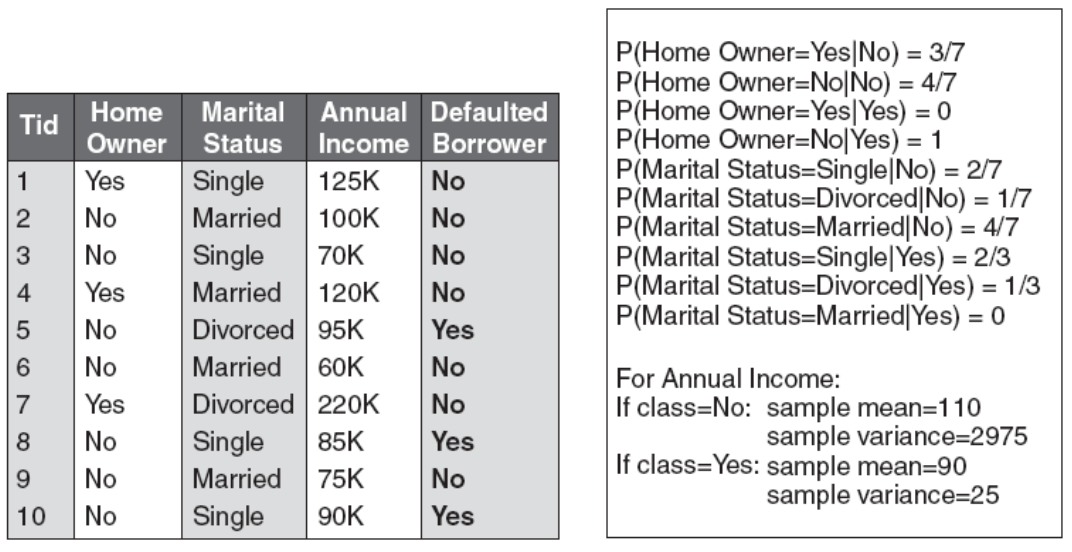
\includegraphics[width=\textwidth]{pics/example.png}
				\end{figure}

				\begin{equation}
				\begin{split}
					P(X|No) = P(Home Owner = No|No) \times P(Status = Married|No) \\
					\times P(Annual Income = 120K|No)
					= \frac{4}{7} \times \frac{4}{7} \times 0.0072 = 0.0024
				\end{split}
				\end{equation}

				\begin{equation}
				\begin{split}
					P(X|Yes) = P(Home Owner = No|Yes) \times P(Status = Married|Yes) \\
					\times P(Annual Income = 120K|Yes)
					= 1 \times 0 \times 1.2 \times 10^{-9} = 0
				\end{split}
				\end{equation}

				\begin{equation}
					P(X|No) > P(X|Yes) \rightarrow X has\:the\:class\:label\:No
				\end{equation}

		\subsection{Problems with naive bayes}

			If you look at the previous example, the calculation of $P(X|Yes)$ was zero
			because one of the attributes had a count of 0. A problem is when we only have 
			a small set of training data, then we probably could get a situation where
			$P(X|Yes)$ = 0 and $P(X|No)$ = 0. What to do now?!

			This problem can be addressed by using the {\bf m-estimate} approach for 
			estimating the conditional probabilities. 

			\begin{equation}
				P(x_{i}|y_{j}) = \frac{n_{c} + mp}{n+m}
			\end{equation}

			where n is the total number of instances from class $y_{j}$, 
			$n_{c}$ is the number of training examples from class $y_{j}$ that takes on the 
			value $x_{i}$, m is a parameter known as the equivalent samle size, and p is a 
			user-specified parameter.

			We can also use the {\bf Laplace} equation:
			\begin{equation}
				P(x_{i}|Y) = \frac{n_{c} +1}{n + c}
			\end{equation}

			where c is the number of classes.

			In the example above we got $P(Status = Married|Yes) = 0$. Using the m-estimate
			with m = 3 and p = 1/3, the conditional probability is no longer zero:

			$P(Marital Status = Married|Yes) = (0+3 \times 1/3)/(3+3)$


		\subsection{Characteristics of Naive Bayes Classifiers}

			\begin{itemize}
				\item They are robust to isolated {\bf noice points} becuase such points are 
				averaged out when estimating conditional probabilities from data. 
				Naive Bayes classifiers can also handle missing values by ignoring the
				example during model building and classification.
				\item They are robust to {\bf irrelevant attributes}. If $X_{i}$ is an irrelevant
				attribute, then $P(X_{i}|Y)$ becomes alomst uniformly distributed. 
				\item {\bf Correlated attributes} can degrade the performance of naive Bayes 
				classifiers because the conditional independence assuption no longer holds 
				for such attributes. 
			\end{itemize}

		\subsection{Bayes Error Rate}

			\begin{equation}
				(\frac{\hat{x} - \overline{x}_1}{s}) = (\frac{\hat{x} - \overline{x}_2}{s} )
			\end{equation}

			Solve this equation for $\hat{x}$ and use it in the next equation for calculating
			the {\bf Bayes error rate}:

			\begin{equation}
				Error = \int_{0}^{\hat{x}} P(Y_{1}|X) dX + \int_{\hat{x}}^{\infty} P(Y_{2}|X)) dX
			\end{equation}

	\section{Support Vector Machine (SVM)}

		Finds a linear {\bf hyperplane} (decision boundray) that will separate the data. 
		The classifier must choose one of these hyperplanes to represent its decision
		boundery, based on how well they are expected to performm on test examples. 

		\begin{figure}[H]
			\subfigure{
				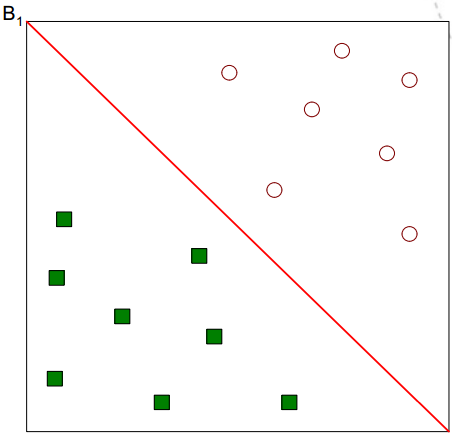
\includegraphics[scale=0.25]{pics/svm1.png}
			}
			\subfigure{
				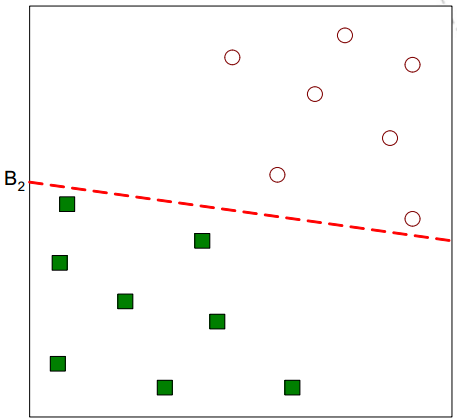
\includegraphics[scale=0.25]{pics/svm2.png}
			}
			\subfigure{
				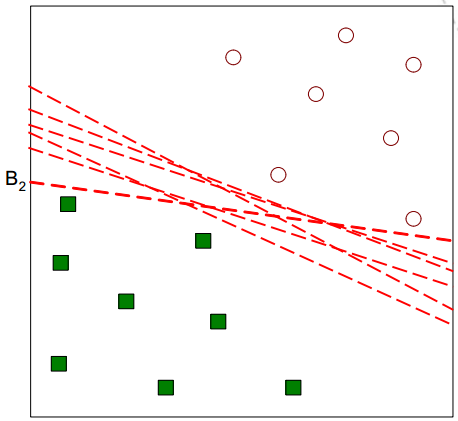
\includegraphics[scale=0.25]{pics/svm3.png}
			}
			\caption{B1, B2, and other solutions}
		\end{figure}

		Which one is better?

		\begin{figure}[H]
			\subfigure{
				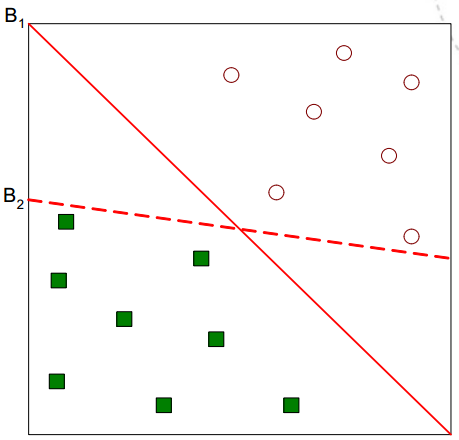
\includegraphics[scale=0.4]{pics/svm4.png}
			}
			\subfigure{
				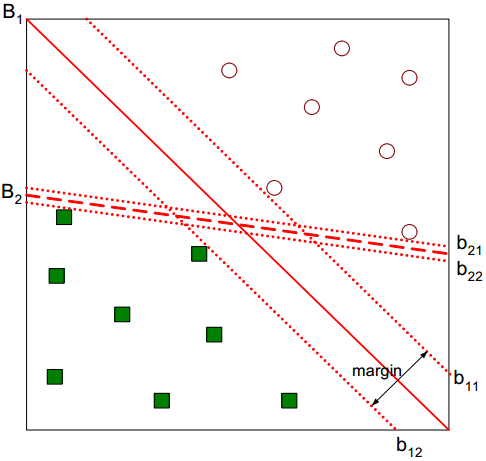
\includegraphics[scale=0.4]{pics/svm5.png}
			}
			\caption{B1 and B2, and the magins}
		\end{figure}

		We want to find hyperplane that maxximizes the margin, therefore we would pick B1. 


